% ==============================================================================
% TCC - Nome do Aluno
% Capítulo 3 - Especificação de Requisitos
% ==============================================================================
\chapter{Especificação de Requisitos e Análise do SCAP}
\label{sec-requisitos}

Considerados um fator determinante para o fracasso ou sucesso de um projeto de \textit{software}, os requisitos desempenham um papel central no processo de \textit{software}. De modo geral, é possível dizer que os requisitos de um sistema incluem restrições sob as quais ele deve operar, restrições que devem ser satisfeitas no seu processo de desenvolvimento, especificações dos serviços que o sistema deve prover e propriedades gerais do sistema~\cite{falbo:er17}.

Os requisitos podem ser definidos como as descrições das restrições operacionais e dos serviços que devem ser providos pelo sistema~\cite{sommerville:es07}. Com relação ao tipo de informação documentada por um requisito, uma classificação é amplamente aceita e de acordo com~\citeonline{sommerville:es07}, os \textbf{requisitos funcionais} são declarações de serviços que o sistema deve prover, descrevendo o que o sistema deve fazer. Já os \textbf{requisitos não funcionais}, descrevem restrições sobre os serviços ou funções oferecidas pelo sistema. Neste contexto, ainda existem as regras de negócio, que definem requerimentos e restrições do negócio, sendo particulares para cada cliente.

Uma tarefa bem útil é representar os requisitos em níveis diferentes de descrição, pois os desenvolvedores, os clientes que contratam o desenvolvimento do sistema e os usuários finais são muito interessados em requisitos, mas possuem expectativas distintas. Assim,~\citeonline{sommerville:es07} realiza a descrição de dois níveis de requisitos:

\begin{itemize}

	\item \textbf{Requisitos de Usuário ou de Cliente:} devem ser de fácil entendimento para clientes e usuários do sistema que não possuem conhecimento técnico. São diagramas intuitivos das restrições e dos serviços esperados do sistema, todos através da utilização de linguagem natural.
	
	\item \textbf{Requisitos de Sistema:} especificam em detalhes as restrições, serviços e funções do sistema, produzindo uma versão melhorada dos requisitos de clientes que os desenvolvedores utilizam para implementar, projetar e testar o sistema. 

\end{itemize}

O capítulo apresenta uma descrição de escopo referente ao SCAP (Sistema de Controle de Afastamento de Professores), assim como os modelos de casos de uso e diagramas de classes que foram levantados anteriormente por~\citeonline{duarte-pg14} e posteriormente analisados por~\citeonline{prado-pg15}. 

\section{Descrição do Escopo}
\label{sec-requisitos-descricao-escopo}

O SCAP surgiu com o objetivo de auxiliar o Departamento de Informática (DI) da UFES no controle e no registro de solicitações de afastamento do seus professores, para que eles possam participar de eventos que acontecem no Brasil e no exterior. Essas solicitações de afastamento necessitam passar por uma série de avaliações para que sejam aprovadas. Elas são avaliadas pelos professores do DI e dependendo do caso, também devem ser avaliadas pela diretoria do Centro Tecnológico (CT) em conjunto com a Pró-reitoria de Pesquisa e Pós-Graduação (PRPPG). Somente após receber a aprovação de todas as instâncias, o afastamento é publicado no Diário Oficial da União e o professor recebe a autorização para participar do evento.     

A Câmara Departamental (composta pelos representantes discentes e pelos funcionários do departamento) fica responsável por avaliar e aprovar as solicitações de afastamento para eventos no Brasil. O chefe do departamento (cargo ocupado por um professor do DI através de um mandato temporário) recebe a solicitação de afastamento pelo email e após dez dias, se nenhum membro da Câmara Departamental for contra ao pedido, o afastamento é aprovado. Assim, para eventos nacionais, o processo permanece dentro do DI.

Para pedidos de afastamento referente a eventos internacionais, um professor (sem parentesco com o solicitante) é escolhido para se tornar relator do pedido. Assim que o relator manda o parecer, o pedido passa por avaliação para aprovação como no caso descrito com eventos que são realizados no Brasil. Para que o pedido seja publicado no Diário Oficial da União, ele deve receber a aprovação do CT e da PRPPG. Entretanto, o SCAP não possui uma integração com os processos do CT e da PRPPG, fazendo com que o controle das tramitações permaneça dentro do DI, restringindo o escopo do sistema.

Com o intuito de automatizar as tramitações das solicitações de afastamento, o SCAP auxilia os professores e secretários do DI, facilitando o processo desde a criação até a aprovação e armazenamento. Com o envio de e-mails automáticos para os envolvidos e com a utilização de formulários para a criação dos documentos necessários, o sistema pode ser considerado fundamental para esse processo.      

\section{Modelo de Casos de Uso}
\label{sec-requisitos-modelo-caso-uso}

As funcionalidades que um sistema deve prover devem ser capturadas e descritas pelos modelos de caso de uso. Na maioria das vezes, um sistema atende a vários atores e por este motivo, analisar a funcionalidade que ele provem como uma única unidade, pode ser uma tarefa complicada. O conceito de caso de uso tem a utilidade de dividir essa funcionalidade em partes mais agradáveis e menores~\cite{olive:cmis07}. Assim, logo após o levantamento de requisitos e da definição do escopo, os atores identificados no sistema SCAP foram apresentados através da Tabela \ref{tabela-atores-scap}.  

\begin{table}[h]
	\centering	
	\vspace{0.5cm}
	\footnotesize
	\caption{Atores do SCAP~\cite{duarte-pg14}}	
	\label{tabela-atores-scap}
	\begin{tabular}{|p{5.0cm}|p{9.0cm}|}  \hline 
 		
 		\rowcolor[rgb]{0.8,0.8,0.8} \textbf{Ator} & \textbf{Descrição} \\\hline 
		
		\textbf{Professor} & Professores efetivos do DI/UFES. \\\hline
		
		\textbf{Chefe do Departamento} & Professores do DI/UFES que estão realizando a função administrativa de chefe e sub-chefe do departamento. \\\hline
		
		\textbf{Secretário} & Secretário do DI/UFES. \\\hline
		
	\end{tabular}
\end{table}

A parte administrativa do sistema fica por conta dos \textbf{secretários}. Eles possuem a responsabilidade de realizar o cadastro dos mandatos dos chefes do departamento, realizar o cadastro dos professores e dos seus respectivos parentescos. Quando surgem pareceres de fora do DI e quando os pedidos de afastamento são finalizados, os \textbf{secretários} também ficam responsáveis pelo controle dessas tarefas.

O SCAP fornece algumas funcionalidades para os \textbf{professores}. Eles podem realizar o cadastro das solicitações de afastamento e realizar uma manifestação contra o afastamento de outro professor, caso ainda esteja dentro do prazo. Além disso, o \textbf{professor} fica responsável por decidir se o DI aprova ou reprova um afastamento no exterior, caso ele seja adicionado como relator do mesmo. 

Se um \textbf{professor} se tornar \textbf{chefe do departamento} através de um mandato, ele deve realizar o encaminhamento de solicitações aos relatores que farão o deferimento de pareceres com relação aos afastamentos internacionais.

O diagrama de casos de uso do SCAP pode ser visualizado através da Figura \ref{fig-requisitos-caso-uso}. Uma pequena descrição dos casos de uso será apresentada nos próximos parágrafos e uma versão mais completa dessa descrição pode ser encontrada em~\cite{duarte-pg14,prado-pg15}.
     
\begin{figure}[h]
	\centering
	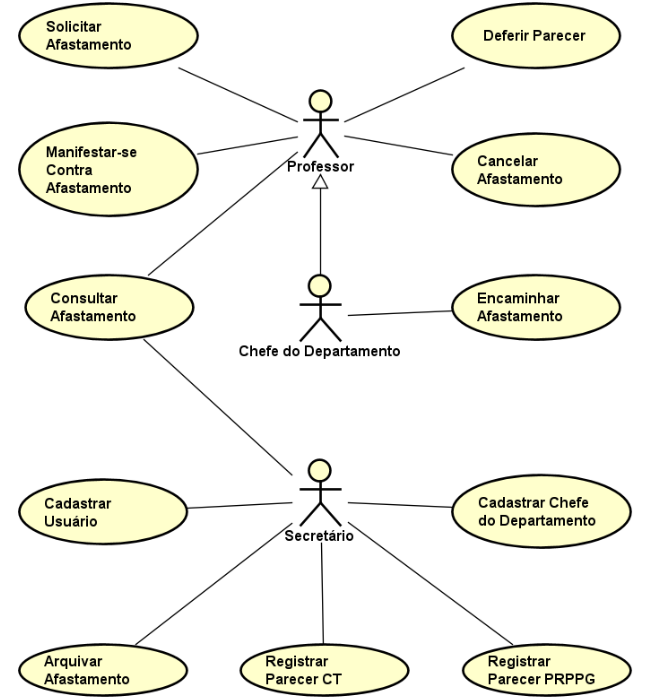
\includegraphics[scale=0.5]{figuras/fig-requisitos-caso-uso} 
	\caption{Diagrama de Casos de Uso do SCAP.}
	\label{fig-requisitos-caso-uso}
\end{figure}

No sistema, um professor realiza o cadastro de um pedido de afastamento por meio do caso de uso \textbf{Solicitar Afastamento}, fornecendo todos os dados que são necessários para realizar a tramitação. Um professor pode cancelar uma solicitação de afastamento utilizando o caso de uso \textbf{Cancelar Afastamento}, realizando a alteração do status para cancelado.

Após escolher um relator para um pedido de afastamento internacional, o Chefe do Departamento pode executar o caso de uso \textbf{Encaminhar Afastamento}. Quando um professor que se tornou relator através da indicação do Chefe do Departamento realizar o cadastro do seu parecer sobre o afastamento, o caso de uso \textbf{Deferir Parecer} pode ser utilizado.

Um professor, um chefe de departamento ou um secretário podem utilizar o caso de uso \textbf{Consultar Afastamento} assim que necessitar obter informações sobre uma solicitação de afastamento. Se um professor for contra a um pedido de afastamento, o caso de uso \textbf{Manifestar-se Contra Afastamento} pode ser utilizado e após o motivo ser cadastrado, uma reunião é agendada para decidir a aprovação ou reprovação da solicitação.

Um secretário realiza o cadastramento de novos professores ou secretários através do caso de uso \textbf{Cadastrar Usuário}, onde é informado todas os dados necessárias. Um secretário também utiliza o caso de uso \textbf{Cadastrar Chefe do Departamento} para especificar o período do mandato do novo chefe do departamento.
  
Quando existe uma solicitação de afastamento internacional, um secretário realiza o cadastro do parecer do Centro Tecnológico e da Pró-Reitoria de Pesquisa e Pós-Graduação por meio dos casos de uso \textbf{Registrar Parecer CT} e \textbf{Registrar Parecer PRPPG}.

O caso de uso \textbf{Arquivar Afastamento} é executado após a tramitação de uma solicitação de afastamento ser realizada, fazendo com que um secretário realize a alteração do status para ``Arquivado''.   

\section{Análise do SCAP}
\label{sec-requisitos-analise-scap}

Fase





   
 
